\chapter{Experimental Setup}
Because of the issues with stimuli generation the experiment setup has not been
employed on live neural tissue.
As a consequence, the current experimental setup is designed to be easy to
modify whenever testing becomes possible and to verify functionality of the rest
of the system.
Unlike traditional reservoir computers there are two orthogonal sets of
parameters to explore which can be divided into neuron-specific and RC-specific
as shown in figure \ref{figParams}.
While it is likely not the case, in order to reduce complexity these two
paratemer sets are viewed as independent which lets us fix one set of parameters
while exploring the other.
\section{Tasks}
Central to each experiment is the task, consisting of a problem for the
reservoir computer to solve and an evaluation function to gauge how well the
problem was solved.
The main task chosen for the reservoir computer is a simple wall avoiding game,
shown in figure \ref{figWall}

\begin{figure}[h!]
  \centering
  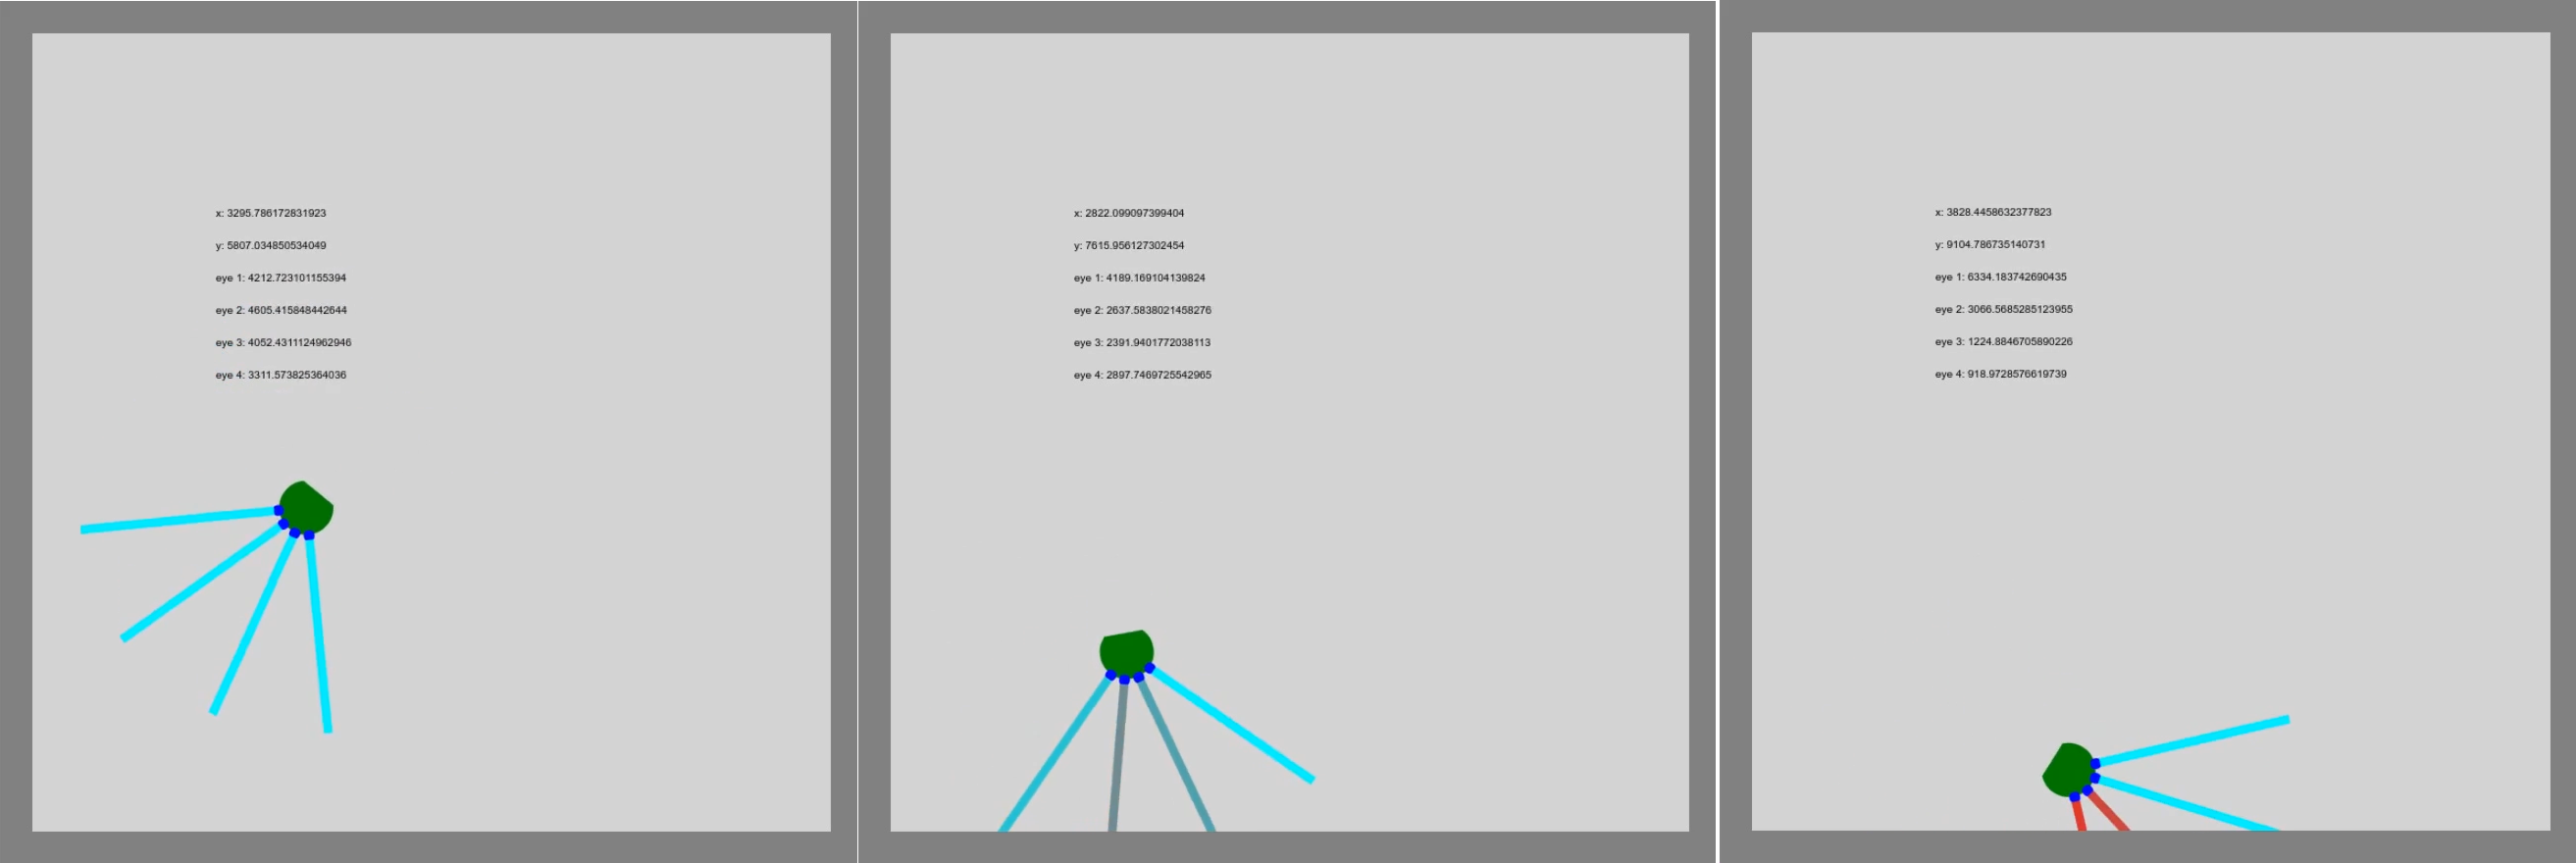
\includegraphics[width=1\textwidth]{fig/TAC/game2.png}
  \caption{A simple conceptual cyborg.}
  \label{cyborgOverviewSimple}
\end{figure}
\cleardoublepage

%%% Local Variables:
%%% mode: latex
%%% TeX-master: "../main"
%%% End: